\documentclass[12]{article}
\usepackage[margin=1.0in]{geometry}
\usepackage[utf8]{inputenc}
\usepackage{titlesec}
\usepackage{physics}
\usepackage[version=4]{mhchem}
\usepackage{graphicx}
\usepackage{siunitx}
\usepackage{cancel}
\usepackage{amsmath}
\usepackage{textcomp}
\usepackage{gensymb}
\usepackage{natbib}
\usepackage{bm}
\usepackage{setspace}

\titleformat*{\subsection}{\normalfont\fontfamily{phv}}
  \titleformat{\subsection}[runin]{\normalfont\bfseries}{\thesubsection.}{3pt}{}
  \titleformat{\subsubsection}[runin]{\normalfont\bfseries}{\thesubsubsection.}{3pt}{}

\title{{\textsc{\Large Nuclear Power Plant Shutdowns: Impact on Particulate Matter and Ozone across the United States}}}
\author{\textsc{Lyssa Freese}
\\\\
Advised by Prof. Noelle Selin}

\doublespace
\begin{document}

\maketitle
\thispagestyle{empty}

\setlength{\leftskip}{1.1cm}
\setlength{\rightskip}{1.1cm}


\bigskip
\bigskip

{\textsc{Abstract.} 
The United States’ future energy mix is likely to transition from its current 19\% reliance on nuclear power. This is due to policy changes and to scheduled shutdowns of nuclear power plants that have reached the end of their lifetime. Given projected growth in demand, the base-load nature of nuclear power, and the intermittency of most renewable resources, fossil fuel-based energy will make up at least part of this deficit and lead to air quality changes and associated health impacts. We develop and validate a generator-level energy grid optimization model, and use its emissions output to drive a chemical transport model, GEOS-Chem. We simulate a hypothetical immediate shutdown of nuclear power plants to test the impact such a policy decision would have on concentrations of ozone and fine particulate matter (\ce{PM_{2.5}}).

When compared to a business-as-usual scenario, the nuclear shutdown scenario leads to a nationwide 50\% increase in \ce{NO_x} emissions and a 45\% increase in \ce{SO2} emissions from coal; and a 40\% increase in \ce{NO_x} emissions from natural gas. We find that the nationwide average \ce{PM_{2.5}} and summertime ozone change +0.4\% and +0.1\%, respectively, with even larger local increases of up to 33\% and 16\%, respectively. Summertime ozone increase in the majority of the northeast and midwest, which are VOC-limited regimes. This suggests that rapidly shutting down nuclear power plants shifts the current generation mix towards dirtier fuel sources, degrading air quality nationwide. Realistically, shutdowns will occur over longer timescales during which new generation will be deployed; this work indicates the importance of prioritizing renewable deployment as new sources of generation in order to reduce these impacts. Importantly, our generator-level energy grid optimization model allows us to assess variations across the scenarios at the local scale, which occur due to a combination of local fuel sources, demand patterns, and chemical regimes.}

\bigskip
\bigskip 
\clearpage
\setcounter{page}{1}

\setlength{\leftskip}{0cm}
\setlength{\rightskip}{0cm}

\section{Introduction}
In 2018, the United States relied on nuclear power for 19\% of electricity generation; by 2050, this is expected to decrease to only 12\% \citep{eia_annual_2020}. This phase-out is due to not only expirations of nuclear power plant licenses, but is accelerated by lower natural gas prices and declining costs of renewables, as well as increasing maintenance costs of nuclear power plants \citep{davis_market_2016}. Nuclear power has played an important role in the U.S. grid over the past few decades, providing energy that has the lowest CO2 emissions (both direct and indirect); and minimal effects on human health due to air pollution \citep{markandya_electricity_2007}, and has been suggested as the future backbone of a low-emissions society \citep{iea_nuclear_2019}. 

Previous work has shown that nuclear shutdowns tend to lead to increased use of fossil fuels, as was seen in the 2012 shutdown of San Onofre’s Nuclear Plant leading to increased use of natural gas, and Tennessee Valley’s Browns Ferry and Sequoyah 1985 shutdowns which were replaced with coal use \citep{davis_market_2016,severnini_impacts_2017}. Fossil fuels have the highest emissions of fine particulate matter (\ce{PM_{2.5}}), \ce{NO_x}, \ce{SO2}, and \ce{CO2} of any energy generating units, a stark contrast to the lack of emissions from nuclear power plants. \ce{NO_x} and \ce{SO2} are precursors for \ce{PM_{2.5}} and \ce{NO_x} is a precursor for ozone, both of which are harmful to human health. Therefore, it is important to understand the air quality and health impacts of the energy transition that will occur over the next few decades. There is currently a lack of literature looking into future emission and health impacts of reducing the role of nuclear power in the U.S. energy market. 

Previous work focuses on the nation-wide health and global climate impact of U.S. energy transitions, particularly the current trend of moving from coal to natural gas \citep{lueken_climate_2016, zhang_climate_2016}, as well as the use of renewables such as wind and solar \citep{millstein_climate_2017}. These studies find \ce{SO2} and \ce{NO_x} reductions from 2016 baselines of up to 90\% and 60\%, respectively, across the United States, with a range of \$20-50 billion reductions in damages to human health \citep{lueken_climate_2016}. 

Prior development and use of energy grid models 1. focus on the economics of future least-cost technology options; 2. take a technology-specific approach; 3. utilize regional average costs, emissions factors, and capacities; or 4. provide detailed modelling of only one energy market \citep{jenkins_enhanced_nodate, epa_ipm_2018}. However, it is important to understand the response of generation and emissions from individual power plants nationwide under different policy scenarios. 

There are two apparent gaps with the current approaches to energy modelling and future emissions assessments. The first is that there is little work looking at the future of nuclear power, specifically shutdowns, and what this will mean for emissions across the United States. The second is that existing work tends to focus on the national level, providing health assessments and emissions changes in national terms. Given the importance of locality to specific plants and their emissions, and the fact that local state and city authorities can play an important role in energy decision-making, we find it important to think about this issue in a way that can be assessed not only nationally, but at a regional and local level as well. 


\section{Methods}

\begin{figure}[!htb]
    \centering 
    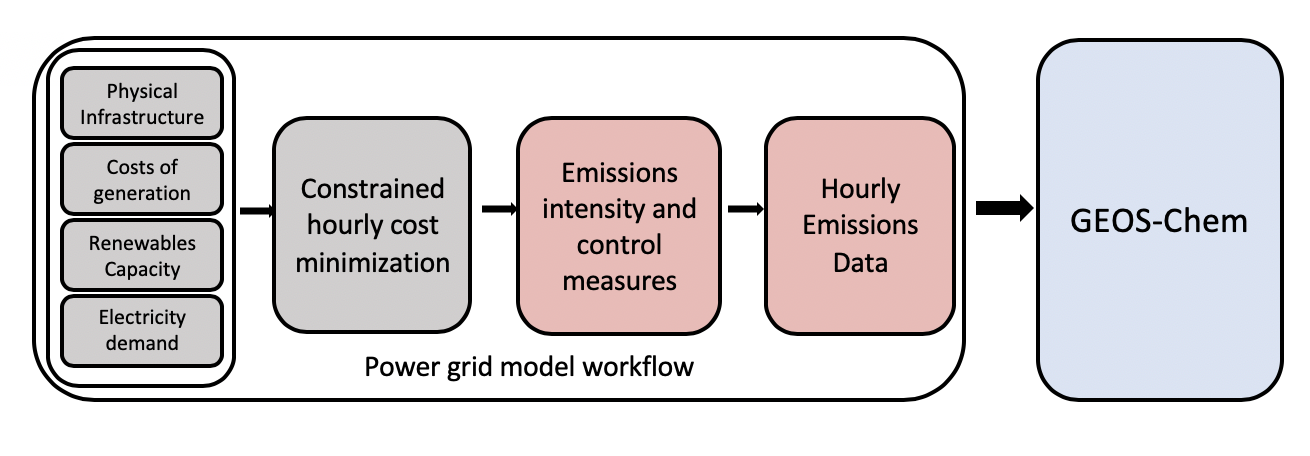
\includegraphics[scale = .5]{US_EGO_flow.png}
    \caption{US-EGO model workflow.}
    \label{fig:my_label}
\end{figure}

\subsection{US Energy Grid Optimization Model (US-EGO).}
US-EGO is a generator-level cost optimization tool. \footnote{This tool was initially developed by Alan Jenn at U.C. Davis for national level assessments. A student in the Aero-Astro department took this initial framework and build a simple model for the U.S., which I assisted in developing.} This tool takes all energy generating units (EGU's) across the United States, their capacity, emission factors (for \ce{CO2}, \ce{SO2}, and \ce{NOx}), and their costs for the year 2016, all of which are based on the EPA's National Electric Energy Data System (NEEDS) model v.5.16 \citep{epa_power_2016}. Separating the nation into NEEDS' 64 regions, we use 2016 transmission data (from the NEEDS data) to allow for transmission between each region, and 2016 loads to simulate demand within each region. As the U.S. energy market functions on a Security Constrained Unit Commitment or Security Constrained Economic Dispatch (SCUC/SCED) optimization model, it is fitting to mimic such an optimization in order to model the market\citep{ela_evolution_2014}. The model then optimizes the use of EGUs such that the load matches generation at every hour in every region. The optimization runs across $t$ time periods with 1. $x_gen$ generation for generator $i$ at cost $c_i$ with $N$ total generators, and 2. $x_trans$ transmission power between regions d and o at cost $c_{o\rightarrow{}d}$. This is run for 8760 hours throughout the year, optimizing at each timestep. \citep{jenn_future_2018}
\begin{equation}
    \min\limits_{x^{gen}, x^{trans}}\sum_{i=1}^{n}\sum_{t=1}^{T} x^{gen}_{i}(t)*c^{gen}_{i}(t) + \sum_{o,d}\sum_{t=1}^{T} x^{trans}_{o\rightarrow{}d}(t)*c^{trans}_{o\rightarrow{}d}(t)
\end{equation}

We restrict transmission such that it mimics the U.S. energy grid, with separation between a western, eastern and Texas grid.

Generation for renewables, such as hydro, solar, and wind are constrained by maximum possible generation profiles (available from the NEEDS data). Additionally, wind and nuclear power are constrained to 85\% and 95\% of their capacity in order to match NEI generation profiles and 
The model returns hourly output of generation. From this we calculate the hourly emissions of \ce{SO2} and \ce{NOx} by:

\begin{equation}
    x^{gen}_{i}EF_i
\end{equation}

Where $EF_i$ is the emissions factor specific to that EGU f
These hourly emissions are merged onto a 0.5\degree by 0.625\degree grid. 

In order to generate the no-nuclear scenario, we remove all nuclear power plants from the possible set of EGUs. In this scenario, generation cannot match the U.S. energy demand in the summertime in the ERC-REST region (eastern Texas), and therefore we close the gap by adding generators that have prohibitive costs such that they are only utilized when the optimization cannot close. These generators have zero emissions, and are there to allow for the optimization to close, and thus we assume partial blackouts in ERC-REST  without nuclear power during those time periods. This in itself is an important outcome of this work, which is that with the current grid, it is unlikely that the U.S. would be able to handle large-scale immediate shutdowns of nuclear power. We understand that realistically, new energy generating units will be developed alongside shutdowns of nuclear power plants, and it is likely much of that will be natural gas or renewables rather than coal, and future work will focus on longer-term scenarios in which new energy development is considered as well.

\subsection{Chemical Transport Model: GEOS-Chem}
We use the GEOS-Chem model \citep{} version 12.6.1 \citep{noauthor_geos-chem_2019} to simulate \ce{SO2}, \ce{NOx}, \ce{PM_{2.5}} and ozone concentrations. We use a global horizontal resolution of 4\degree x 5\degree to create boundary conditions for a nested North American run with horizontal resolution of 0.5\degree by 0.625\degree between 140\degree - 40\degree W and 10\degree - 70\degree N. We run full-chemistry in the troposphere only, with 47 vertical levels. Our spin-up is four months, and we analyze daily concentration outputs for the year of 2016. GEOS-Chem version 12 has a number of improvements that reduce the high nitrate bias seen in previous versions of GEOS-Chem \citep{walker_simulation_2012}, including 1. improved dry deposition of \ce{HNO_3} at cold temperatures \citep{jaegle_nitrogen_2018}, 2. updates to ISORROPIA, the thermodynamic model for inorganic aerosol formation to version 2.2 \citep{fountoukis_isorropia_2007}, and 3. improved treatment of heterogeneous \ce{NO_2}, \ce{NO_3}, and \ce{N_2O_5} chemistry in aerosols and clouds.

We run four GEOS-Chem simulations with different U.S. EGU emission inputs: default, e-grid, US-EGO, and no-nuclear. The default simulation takes the standard GEOS-Chem U.S. EGU emissions files, which are taken from the National Emissions Inventory (NEI) 2011 emissions scaled to the year 2013. The e-grid simulation utilizes the EPA's Emission and Generation Resource Integrated Database (e-grid) \citep{epa_emissions_2016} \ce{SO2} and \ce{NOx} emissions gridded onto a 0.5\degree by 0.625\degree grid. The US-EGO simulation uses the emissions profiles created through the US-EGO model, and the no-nuclear scenario uses emissions profiles created through the US-EGO model in a no nuclear scenario. 

\begin{figure}
    \centering
    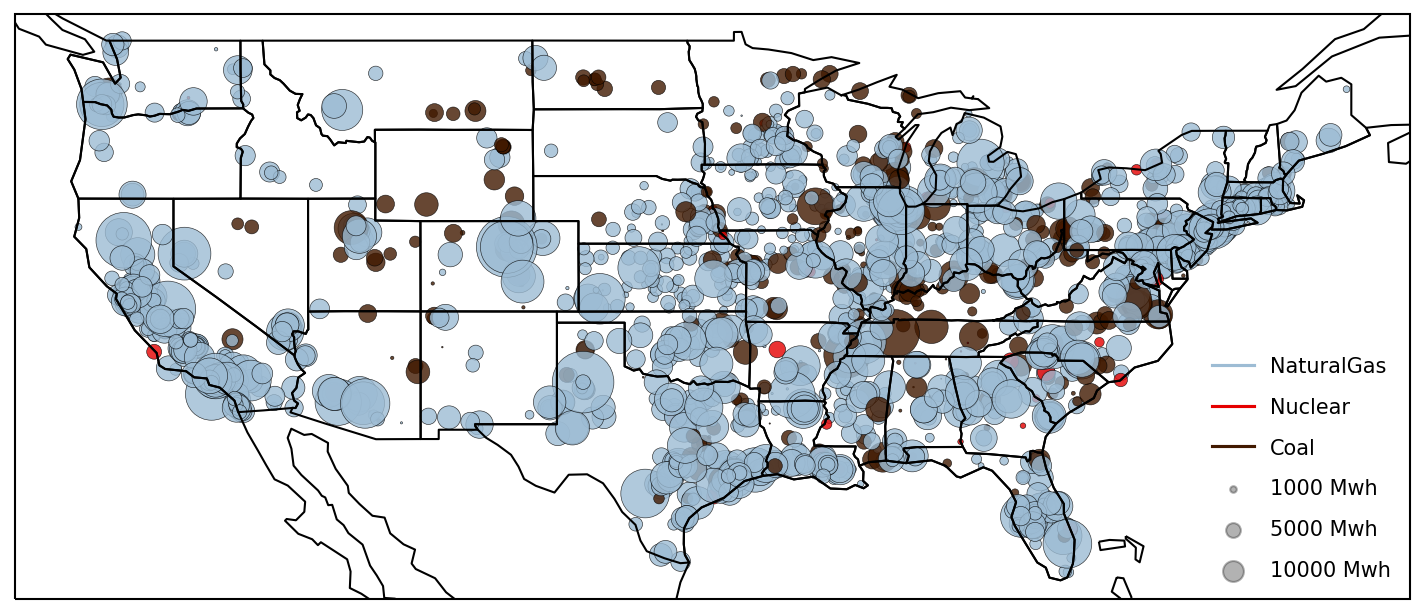
\includegraphics[scale=0.4]{ego_nonuclear_project/Figures/plants_normal.png}
    \caption{Spatial maps of coal, nuclear and natural gas power plants across the U.S.} 
    \label{fig:plants}
\end{figure}

\section{Results}
\subsection{Model Validation}

In order to evaluate the model, we compare our emissions output to that of the EPA's e-grid, and the NEI 2011 data, scaled to the 2013 values as is the default in GEOS-Chem \citep{geos-chem_epanei11_2019}. The NEI is the EPA's comprehensive estimate of air pollutants from point, nonpoint, road and nonroad sources, and is created every three years \citep{us_epa_national_2015}. E-grid is the EPA's database on environmental characteristics of electricity generating sources in the United States, providing generation data by EGU, and is available yearly \citep{us_epa_emissions_2015}. Thus these databases directly provide an opportunity to evaluate the model both before and after running it through GEOS-Chem. 

We compare e-grid generation by each region and fuel type with our model emissions before running it through GEOS-Chem. 
Figure \ref{fig:emissions_region}) shows these results, which have a Pearson's correlation coefficient of .84. Additionally, we compare GEOS-Chem output from the e-grid, NEI and normal model runs to see what regions differ in their concentrations of pollutants. This can be seen in Figure \ref{fig:obs_model}, where the ranges of values for each pollutant are shown for each simulation.

We also compare the annual mean GEOS-Chem concentrations of each model run to two on-the-ground observational networks: the EPA Air Quality System (AQS) monitoring data for 2016 \citep{us_epa_daily_2016} and the IMPROVE network \citep{malm_spatial_1994}. We compare to AQS observations for \ce{PM_{2.5}}, \ce{NO_2}, \ce{SO_2} and ozone; and to IMPROVE observations for \ce{PM_{2.5}}, sulfate, nitrate (Figure \ref{fig:obs_model}). We find the squared correlation ($r^2$) and normalized mean bias (NMB) for every region and season between the normal scenario and observations of each pollutant. We calculate a normalized mean bias (NMB) as $\frac{\sum(M_i - O_i)}{\sum(O_i)}*100$, where i is the seasonal mean at each observational site.


\begin{figure}
    \centering
    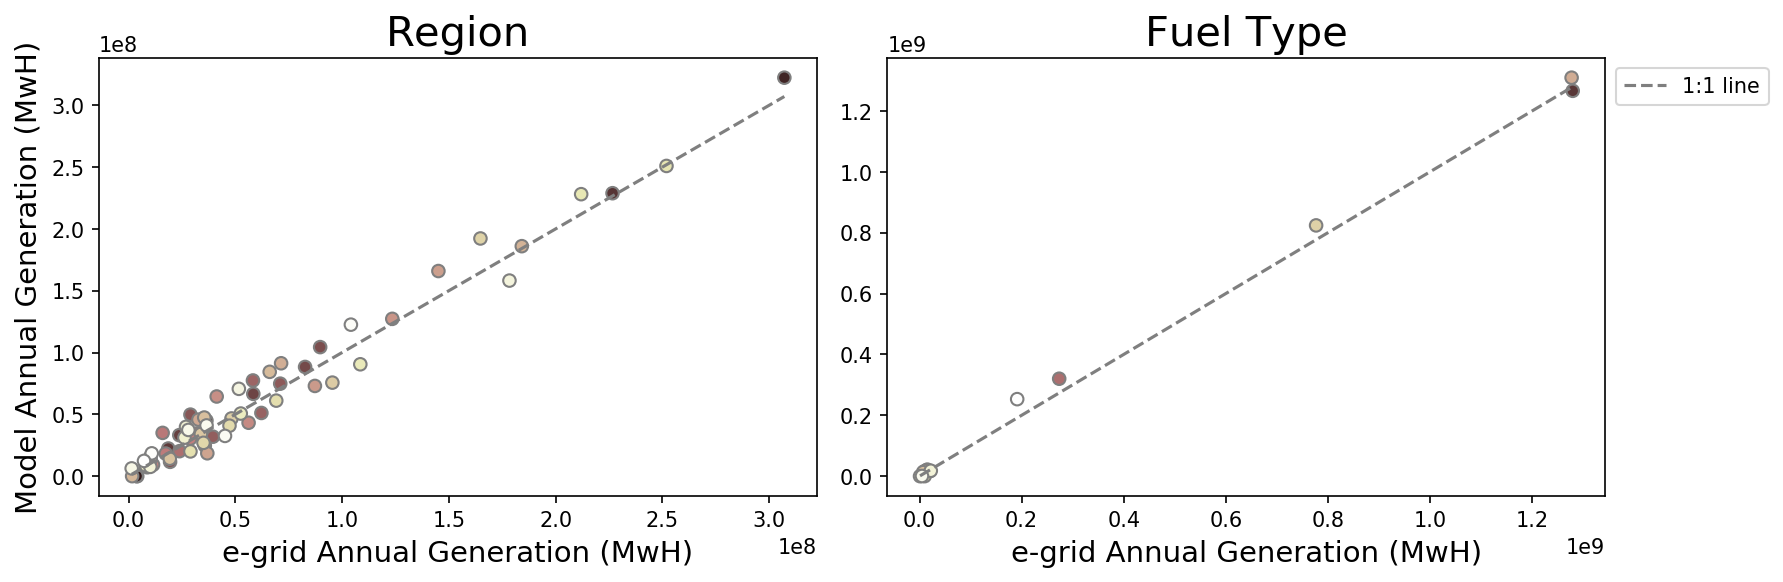
\includegraphics[scale=0.3]{ego_nonuclear_project/Figures/egrid_model.png}
    \caption{Scatterplot of the annual generation by both region and fuel type. We compare generation of e-grid and the model as e-grid's raw output data provides annual generation, rather than annual emissions.} 
    \label{fig:emissions_region}
\end{figure}

For \ce{NO_2}, we find an $r^2 = 45\%$ and a bias low ($NMB = -8\% to -50\%$) depending on the region and season. We find the smallest bias between model \ce{NO_2} and observations during the summer months, in particular, in the Northeast. Ozone has an $r^2 = .07$, with a NMB ranging from -24\% to 23\%. \ce{SO_2} has a low bias (negative NMB) in the model in the northwest, southwest, and midwest, but a high bias (positive NMB) in the northeast and southeast. Sulfate is biased high (NMB = 112\% and 167\% during winter and summer, respectively) in the northwest, as well as in the summertime in the northeast (NMB = 91\%). Our nitrate is biased extremely high compared to the observations, at values of up to NMB = 3700\% in the northeast during the summertime. This bias is particularly high in summer throughout all regions relative to wintertime. However, this does not directly translate to bias in the \ce{PM_{2.5}}, as between both the IMPROVE and AQS data, we find model bias to have a maximum of 253\% in the summertime in the Northeast. This nonlinearity is further explored below through the use of ISORROPIAII. 

This correlation and bias is in line with previous work \citep{holt_changes_2015} on an earlier version of GEOS-Chem, as well as work on other chemical transport models \citep{simon}, although both our nitrate and sulfate bias in the summer time are found to be much higher.

\begin{figure}
    \centering
    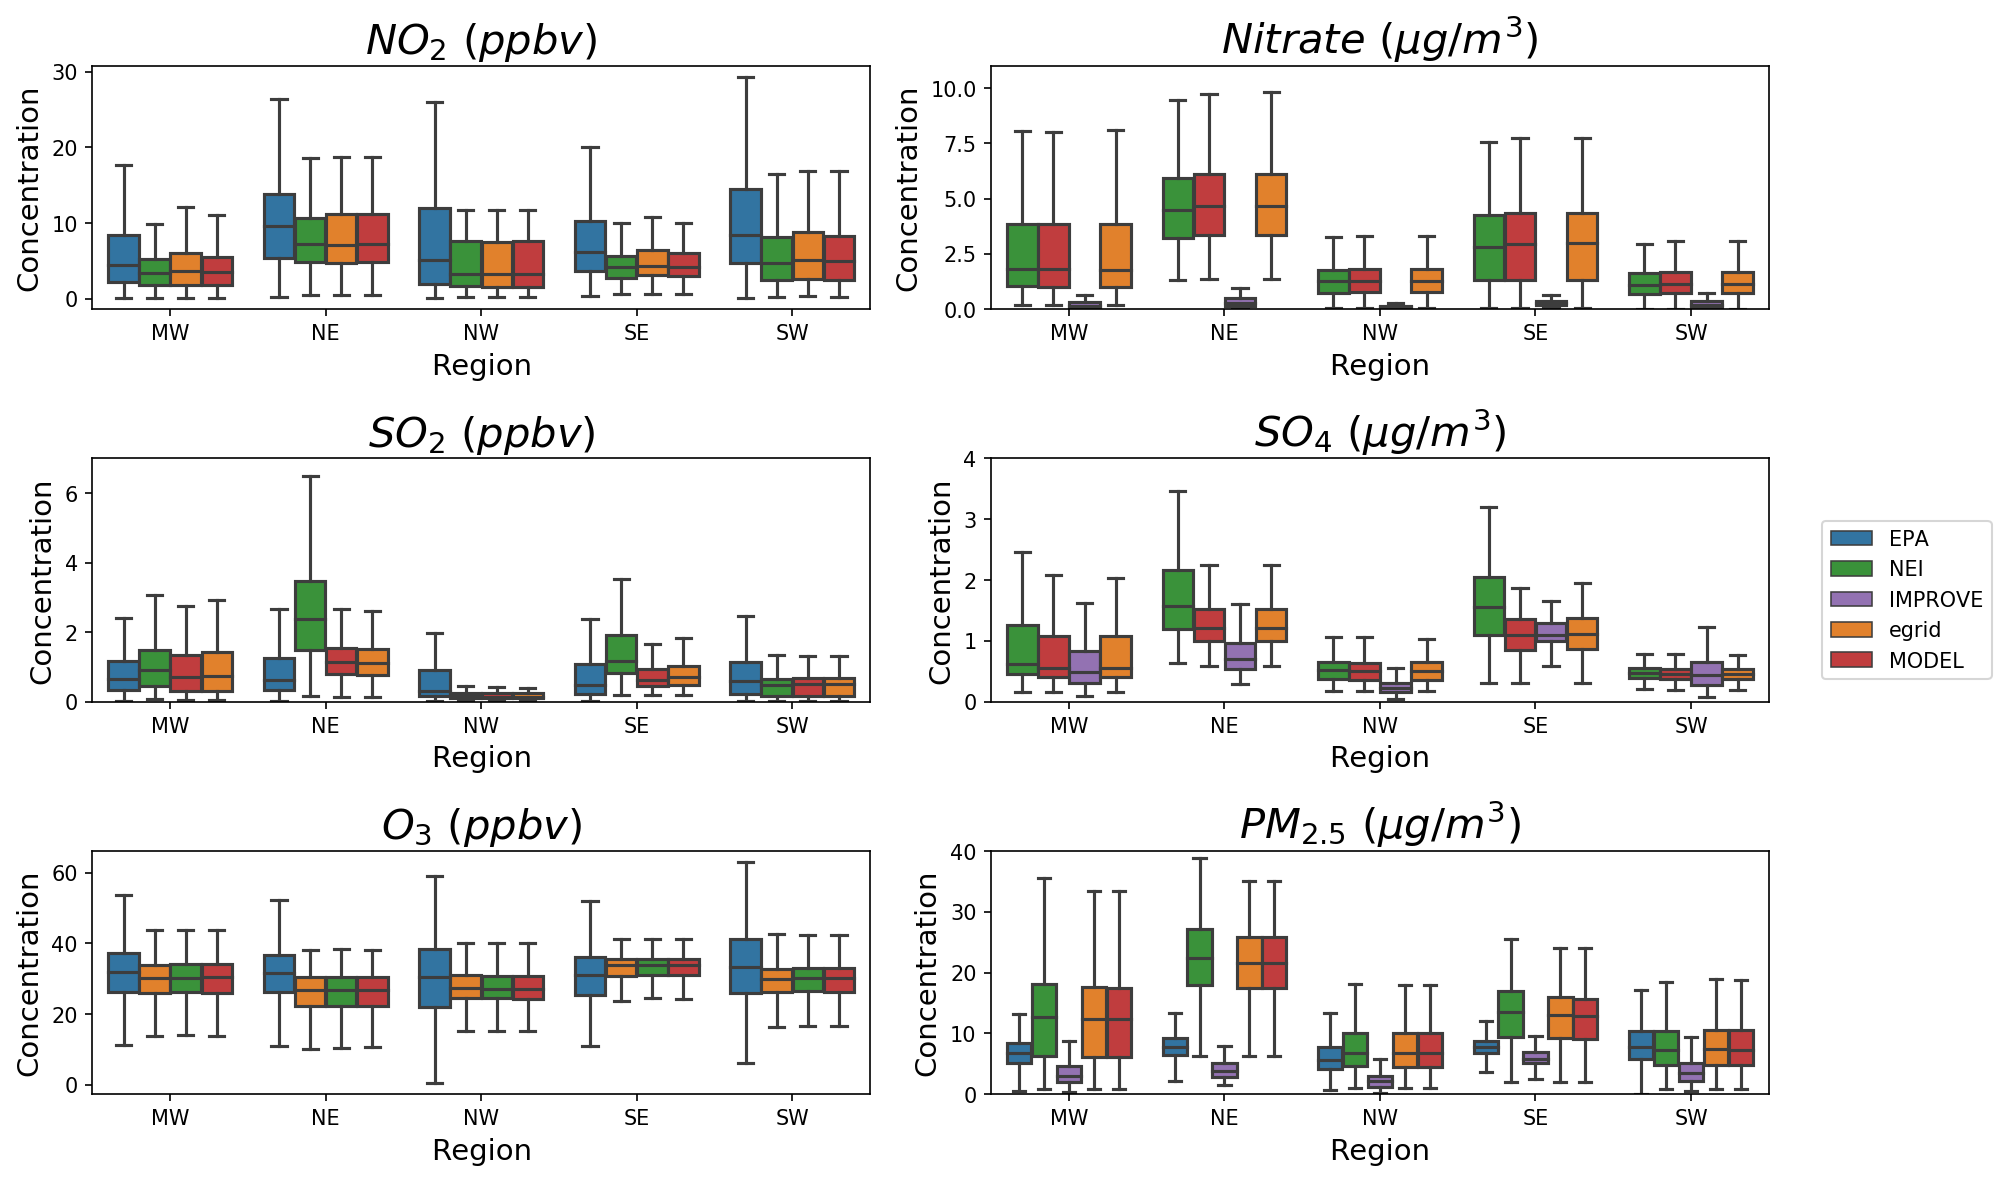
\includegraphics[scale=0.5]{model_validation/Figures/obs_boxplots.png}
    \caption{Box plots of monthly mean observations at each site within a given region for both IMPROVE and AQS sites compared to monthly mean model simulated values at the location nearest each observational site.} 
    \label{fig:obs_model}
\end{figure}


\subsection{Ozone and \ce{PM_{2.5}} impacts of a no-nuclear scenario}
Here we look at the differences between the no nuclear and normal scenarios in the summer, June, July and August (JJA) and winter, December, January, February seasons (DJF). 

We find that in the no nuclear case, \ce{NO_x} emissions increase by 50 \% for coal and 40\% for natural gas, and \ce{SO_x} emissions increase by 45\% for coal. These emission changes are highest in regions that had more nuclear power plants, as well as larger reliance on coal and natural gas, such as the northeast, southeast, and midwest (Figure \ref{fig:emissions_nonuc}). 

\begin{figure}
    \centering
    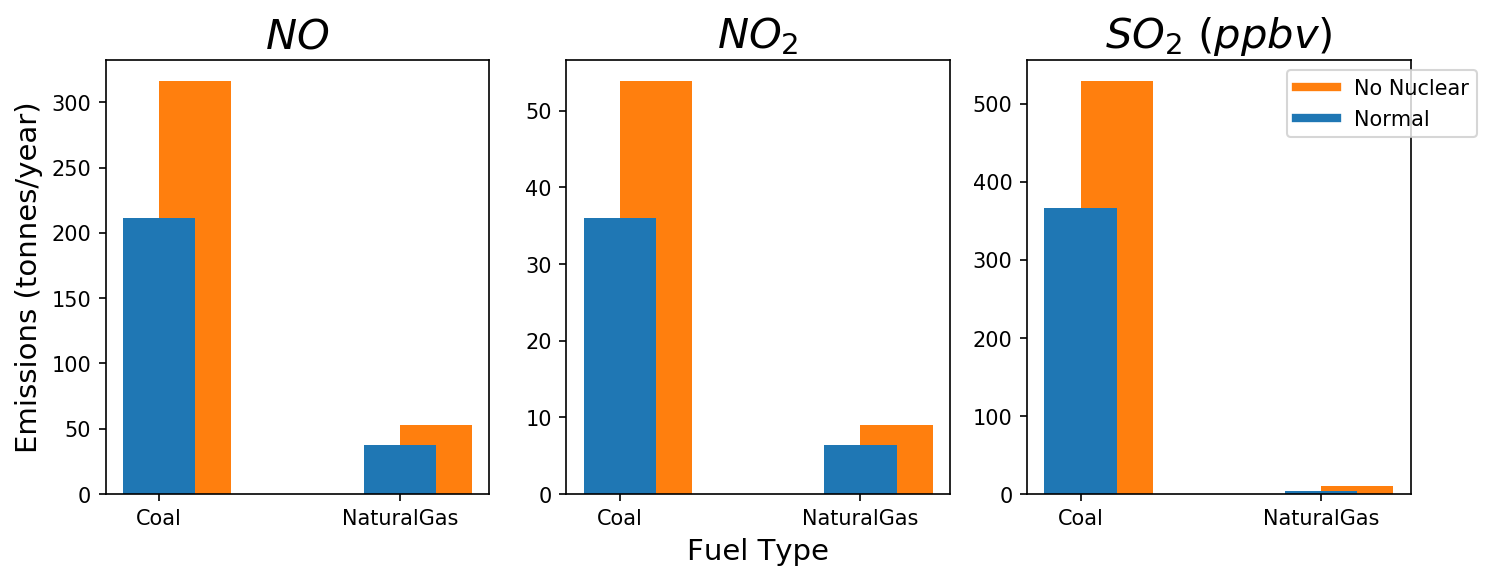
\includegraphics[scale=0.4]{ego_nonuclear_project/Figures/emissions_fueltype.png}
    \caption{Change in emissions by fuel type between the no nuclear scenario and nuclear scenario. We } 
    \label{fig:emissions_comp}
\end{figure}

\begin{figure}
    \centering
    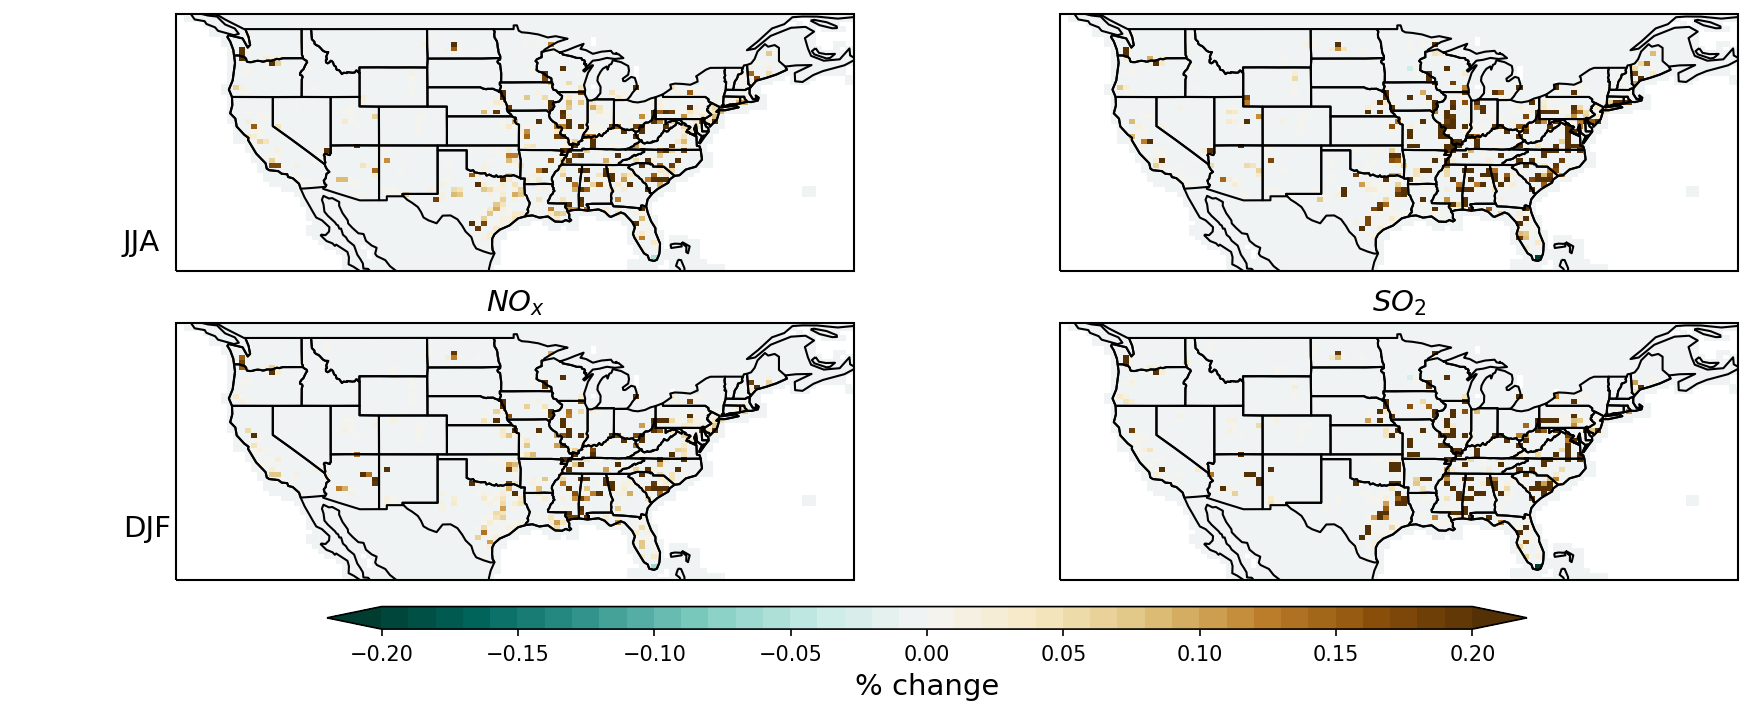
\includegraphics[scale=0.4]{ego_nonuclear_project/Figures/nox_so2_emissions.png}
    \caption{Spatial maps of percent differences in \ce{NO_x} and \ce{SO_2} emissions between our normal and no nuclear scenario. We find increase of over 20\%, much of which occurs in the northeast, southeast, and midwest regions.} 
    \label{fig:emissions_nonuc}
\end{figure}

Differences between the two scenarios in \ce{SO2} and \ce{NOx} concentrations are similar in the summer and winter, with the largest differences occurring in the eastern Midwest, Northeast and Southeast, as seen in Figure \ref{fig:summer_winter_dif}. We find increases in both for a no nuclear scenario when compared to our normal scenario. The regions in which concentrations increase are also regions in which there is a much larger reliance on nuclear power in the normal scenario, as well as shift to reliance on coal in the no nuclear scenario, as can be seen in Figure \ref{fig:plants}. \ce{NOx} concentrations increase by up to 40 ppb (a 1000\% increase) in Western Pennsylvania during the wintertime, and \ce{SO2} concentrations increase by up to 18 ppb (a 3700\% increase) along the Pennsylvania-Ohio border during wintertime. 
\begin{figure}
    \centering
    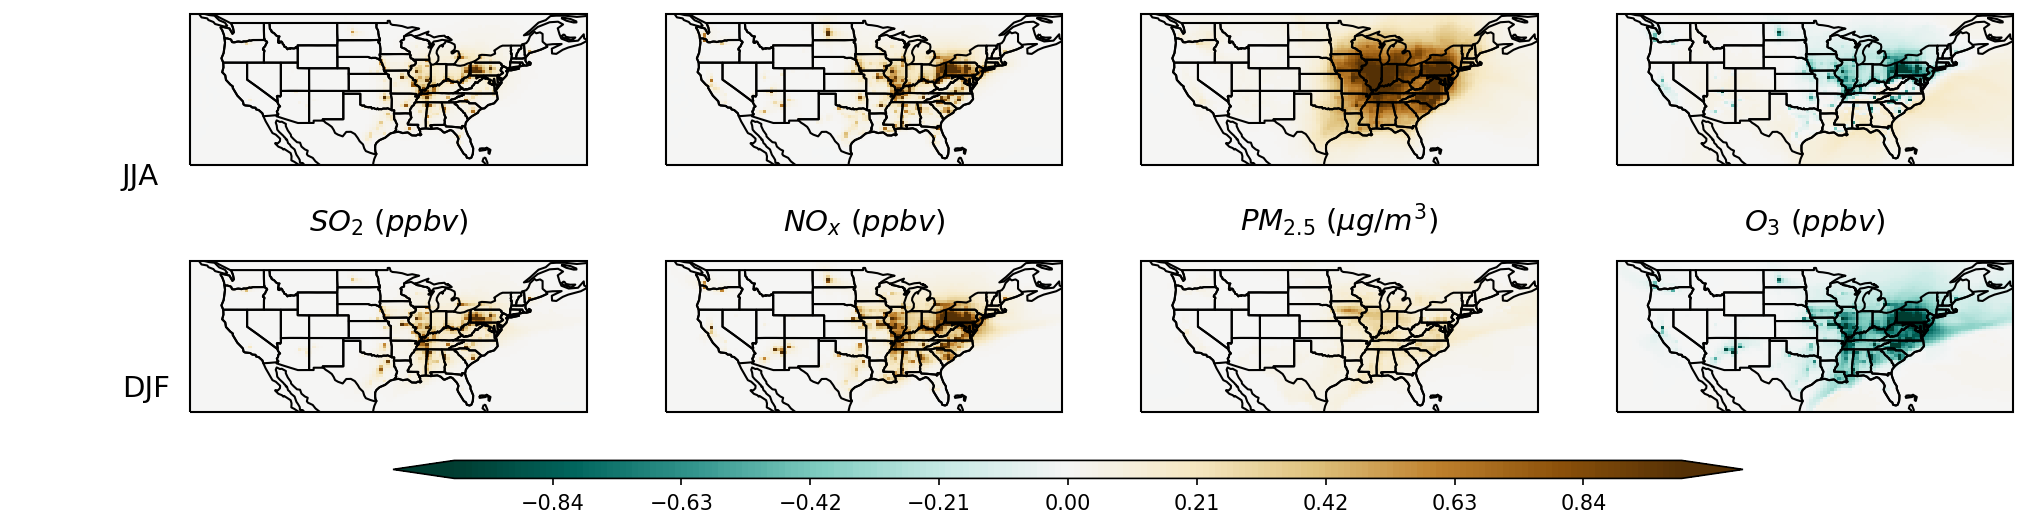
\includegraphics[scale=0.5]{ego_nonuclear_project/Figures/summer_winter_national_dif.png}
    \caption{Spatial maps of summer (JJA) concentration differences between scenarios (no nuclear - normal). We see the largest differences in \ce{NO_x} and \ce{SO_2} concentrations in the Northeast, leading to large differences in \ce{PM_{2.5}} and ozone in the region as well.} 
    \label{fig:summer_winter_dif}
\end{figure}

There are overall increases in both summertime and wintertime \ce{PM_{2.5}} concentrations across the United States when nuclear power plants are shut down, with changes of up to 10 $\mu g/m^3$ occurring in June in eastern Missouri. Increases in \ce{PM_{2.5}} during the summer time are an average of .04 $\mu g/m^3$ greater than during the winter. Particularly, in the central-western Pennsylvania, the summer time \ce{PM_{2.5}} difference is up to 1.2 $\mu g/m^3$ greater than that in the winter. 

Summertime ozone, on the other hand, decreases throughout the Northeast, with slight increases in the Southeast and western Midwest regions. Maximum ozone increases occur along the South Carolina-Georgia border with increases of 1.7 ppb. Decreases are largest in the Northeast, particularly along the Pennsylvania-Ohio border, decreasing by up to 21.8 ppb. 

\subsection{Ozone Regimes}
Based on \cite{jin_evaluating_2017}, we calculate a surface ratio of formaldehyde to \ce{NO_2} (FNR), which we use to evaluate the surface ozone production regime of each grid cell. For ratios < 0.5, we assume a VOC limited regime, for ratios > 0.8, we assume a \ce{NO_x} limited regime, and in between is transitional. In VOC limited regimes, an increase in \ce{NO_x} will actually contribute to decreased levels of ozone, as VOCs are fully saturated and any additional \ce{NO_x} will contribute to suppression of ozone formation. This is what occurs throughout the Northeast and eastern Midwest regions when we increase \ce{NO_x} in the no nuclear scenario. On the other hand, in \ce{NO_x} limited regimes, such as rural areas in the Southeast and Northeast, we find increased levels of \ce{NO_x} leading to increases in ozone, as the VOCs are not fully saturated and any additional \ce{NO_x} will contribute to the formation of ozone.  

\begin{figure}
    \centering
    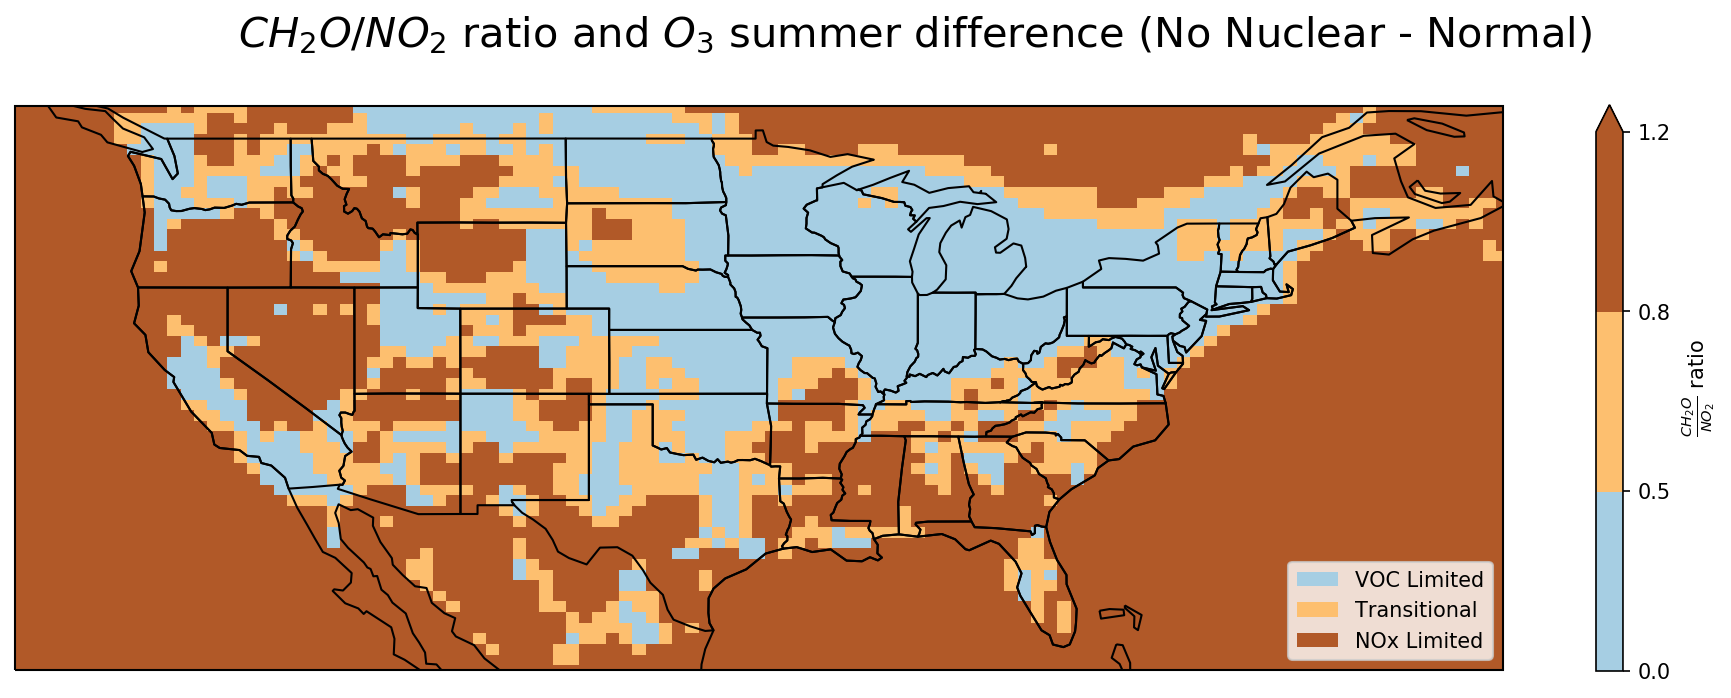
\includegraphics[scale=0.4]{ego_nonuclear_project/Figures/summer_regime_national_ratio.png}
    \caption{Spatial maps of summer (JJA) FNR} 
    \label{fig:summer_FNR}
\end{figure}
\subsection{\ce{PM_{2.5}} Sensitivities}
As we find in the model validation, GEOS-Chem has a high nitrate bias in the Northest, so we expect this to impact our \ce{PM_{2.5}} concentrations in both the no nuclear and normal scenarios. Here we discuss the implications of the bias that we previously described, and explain its role in this work.

We utilize an offline version of ISORROPIAII, which allows us to look at inorganic particulate matter formation as a function of temperature, relative humidity, nitrate, sulfate, ammonia, chlorine, potassium, magnesium and calcium \citep{fountoukis_isorropia_2007}. We use regional and seasonal mean sulfate, temperature, and relative humidity values from our normal scenario model runs, and set a range for total \ce{NH3} and total nitrate to obtain Figure \ref{fig:isorropia}, which provide an understanding of the sensitivity of inorganic \ce{PM_{2.5}} formation to both ammonia and nitrate concentrations. In the winter season, there is a clear delineation of where there is enough \ce{NH3} to neutralize both \ce{NO_3^-} and \ce{SO_4^{2-}}. Above this line, changes in nitrate have no effect on the formation of inorganic \ce{PM_{2.5}}. Below this line \ce{PM_{2.5}} is strongly dependent on nitrate concentration. 

We compare this to the seasonal average total nitrate and total \ce{NH3} from IMPROVE observations at each station, and to our normal and no nuclear scenario model outputs interpolated to each station. As can be seen, our nitrate values are much higher in the model data than in the IMPROVE observational data, while the \ce{NH3} values fall within a similar range. In the wintertime case for the northeast, southwest, and midwest, as well as the higher \ce{NH3} ranges for summertime in the northeast and midwest, our inorganic \ce{PM_{2.5}} concentrations not only fall clearly below the point where \ce{NH3} neutralizes both \ce{NO_3^-} and \ce{SO_4^{2-}}, but also has values that differ from our observations because of these high nitrate values. This causes our \ce{PM_{2.5}} concentrations to also be biased high, such that at a similar \ce{NH3} concentration, they do not fall into the same range of \ce{PM_{2.5}} concentrations. Both of our scenarios do, however, fall into similar \ce{PM_{2.5}} formation regimes for each observational point, which means that our changes in \ce{NO_x} and \ce{SO_2} are not causing any nonlinearities to arise in the no nuclear scenario as compared to the normal scenario. Thus we can compare across the two cases to understand the differences, with the understanding that the absolute values of \ce{PM_{2.5}} will be biased high.

\begin{figure}
    \centering
    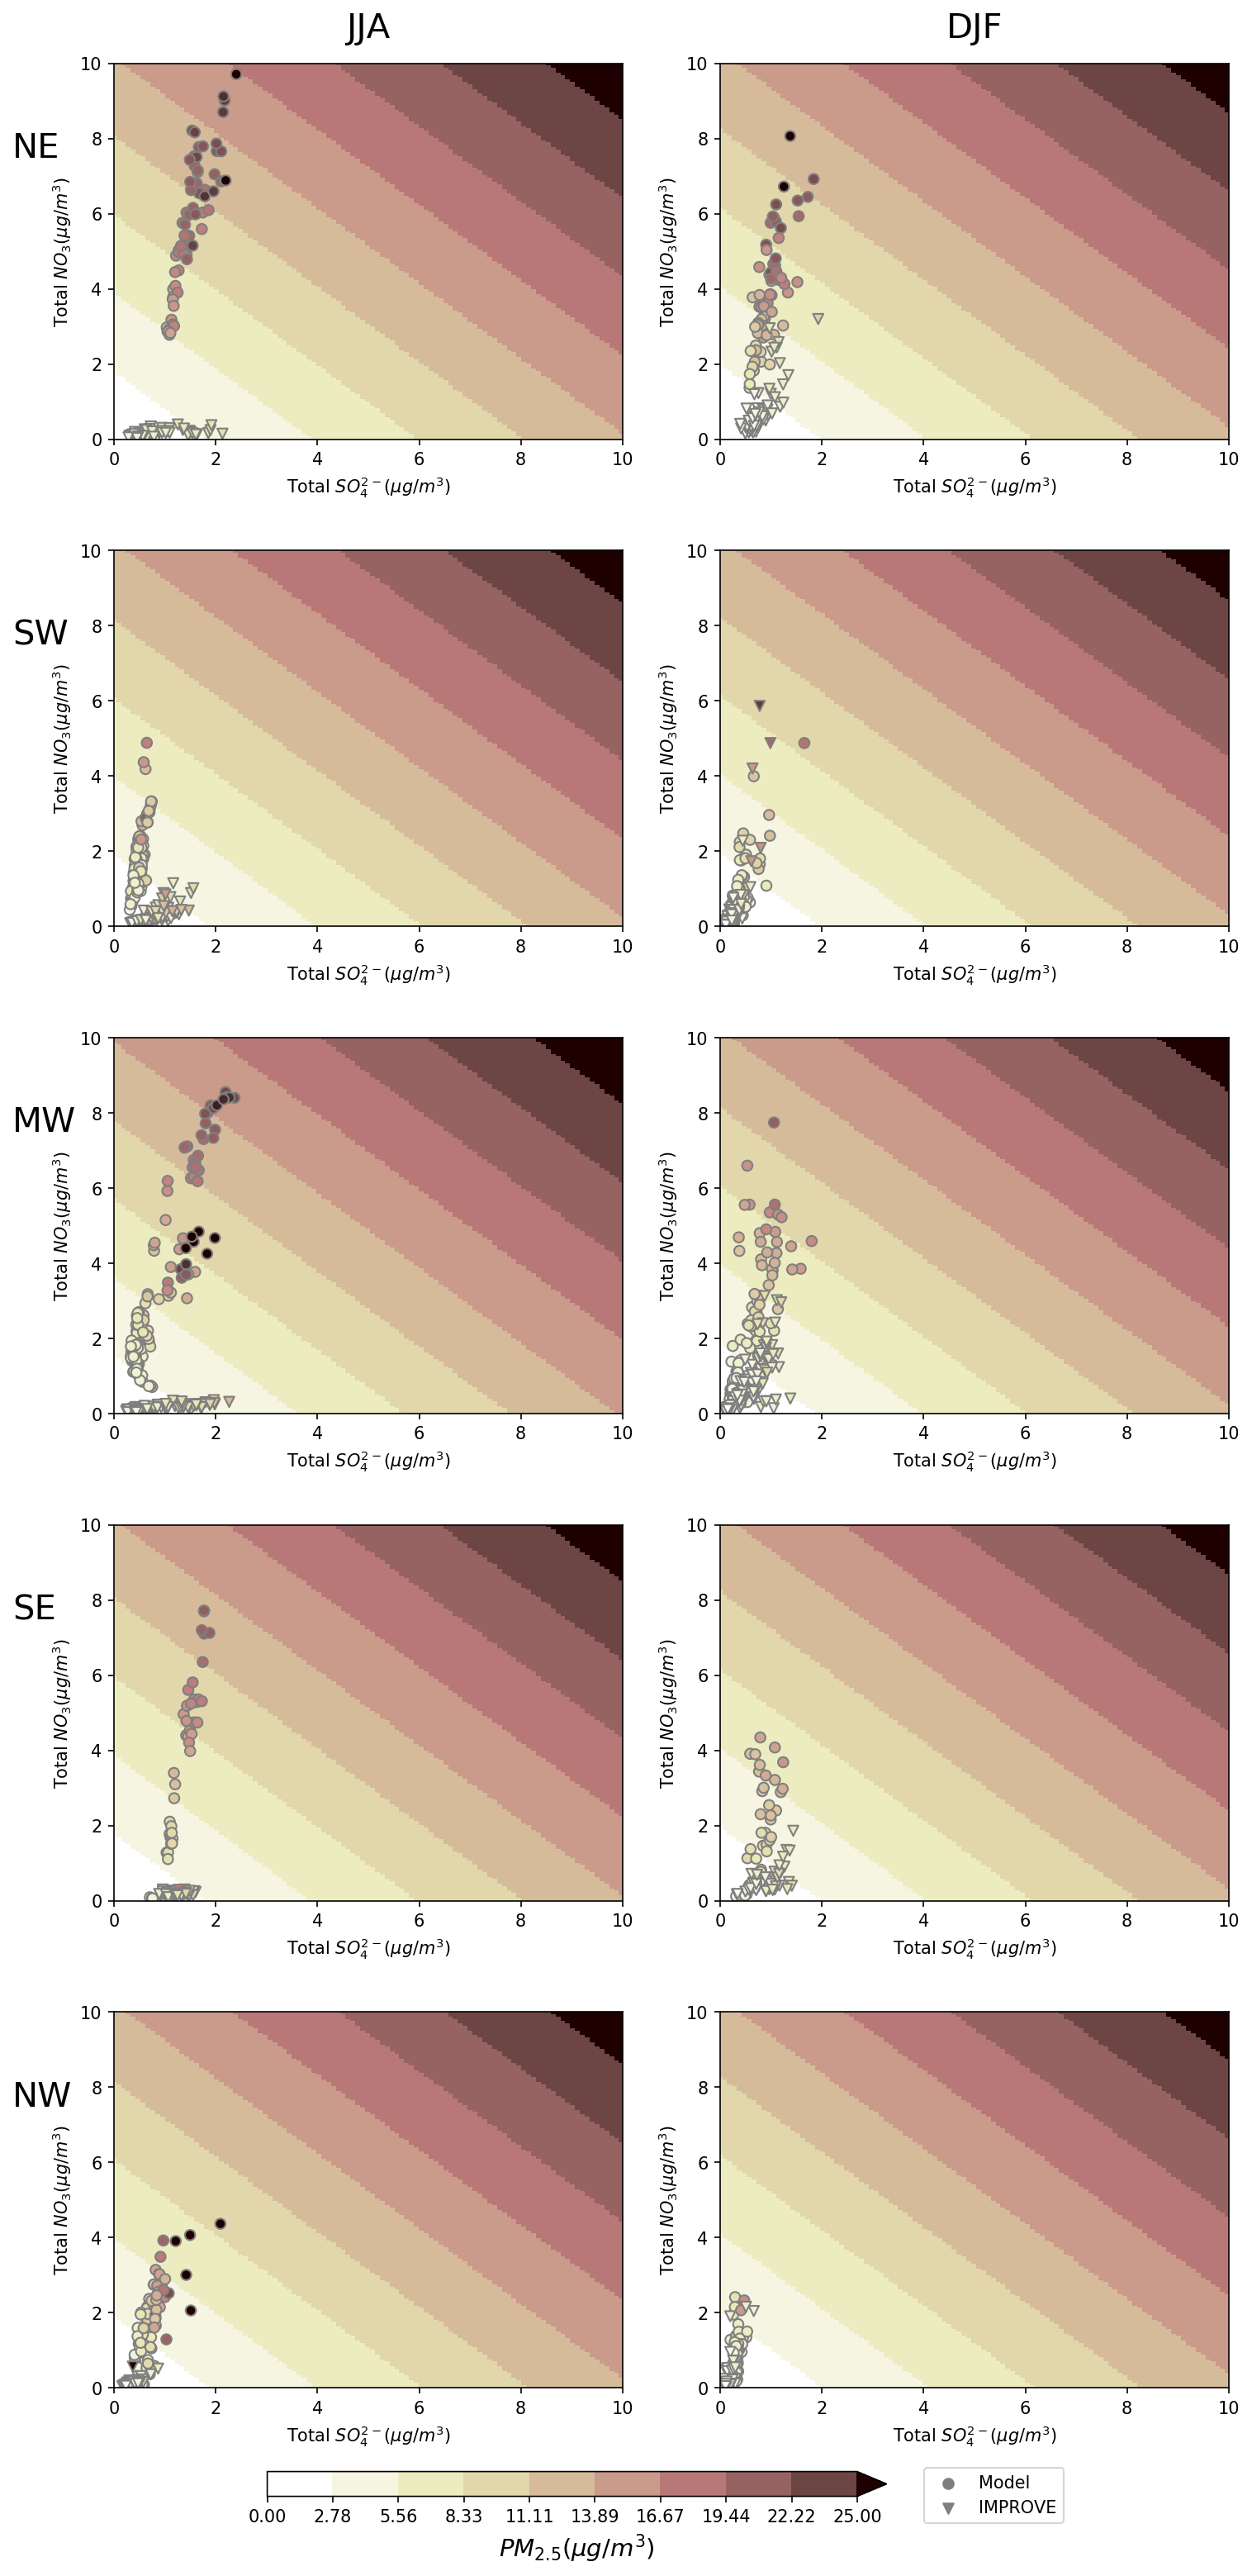
\includegraphics[scale=0.4]{ego_nonuclear_project/Figures/isorropia_obs_plot.png}
    \caption{Plots of standalone ISORROPIAII output for each region based on regional average temperature, relative humidity, and ammonia concentrations. Plotted on top are annual mean observational values for sulfate, nitrate, and \ce{PM_{2.5}}.} 
    \label{fig:isorropia}
\end{figure}

\section{Discussion}

Overall, we find that under a no nuclear scenario, fossil fuel energy generation increases by 43\% for coal and 21\% for natural gas. This drives large increases in both \ce{SO_2} emissions and \ce{NO_x} emissions, which we find to increase up to 50\% for coal and 40\% for natural gas. As coal is largely concentration in certain regions, particularly in the rust-belt states of Ohio, Pennsylvania and Indiana, this shift will lead to emissions increases that are unequal across regions throughout the U.S.

As many of these regions already have high levels of \ce{NO_x}, we find decreases in summertime ozone across the majority of the northeast. The southeast and western portion of the midwest see slight increases in ozone, but not enough to exceed ozone standards. These decreases in ozone, however, are countered by increases in \ce{PM_{2.5}} across an even larger portion of the northeastern U.S., extending into the entire southeast and the midwest. These increases of up to 10 $\mu g/m^3$ can have significant impacts on human health \citep{burnett_global_2018}. Further quantification of the health impacts of both changes in ozone and \ce{PM_{2.5}} can help with a better understanding of the overall impact of shutdowns on human health. 

We use ISORROPIAII as a standalone model to understand the sensitivity of \ce{PM_{2.5}} to nitrate bias in the GEOS-Chem model. Although we find high bias in both our nitrate and \ce{PM_{2.5}} concentrations, particularly in the northeast, this bias is present in both the normal and no nuclear scenario, allowing us to compare across scenarios. Recent changes to GEOS-Chem that improve nitric acid deposition have been shown to reduce the bias in nitrate to reasonable levels \citep{luo_revised_2019}, and reassessment under this model might provide a more accurate understanding of the absolute values of \ce{PM_{2.5}} in each scenario.

With this understanding, it is clear that nuclear shut downs will lead to increased coal and natural gas use as well as \ce{PM_{2.5}} concentrations, while decreasing ozone. This is amplified in regions with both large numbers of nuclear plants and fossil fuel plants, such as the northeast, southeast, and midwest. These impacts do not even look at the \ce{CO_2} emission changes that will occur due to this shift, which is an important aspect that should also be considered. It is important for national and local policies on the future of nuclear power plants to take these impacts on both local and regional air quality into account.


\pagebreak
\bibliographystyle{apalike}
\bibliography{references.bib}

\end{document}

